\section{Setup}
Before beginning, players must decide how many rounds to play. 
We recommend 4 rounds for 2 players, and 8 rounds for 3-4 players, but feel free to change it up.
\subsection{2 Players}

\begin{enumerate}
    \item Flip all the dominoes face-down onto the table and give them a good shuffle.
    \item Arrange all the dominoes in 5 columns of 11
    \item Flip over the middle domino in each column.
\end{enumerate}

\subsection{3--4 Players}

\begin{enumerate}
    \item Flip all the dominoes face-down onto the table and give them a good shuffle.
    \item Arrange all the dominoes in 7 columns of 13
    \item Flip over the middle domino in each column.
\end{enumerate}

\begin{figure}[ht]
\centering
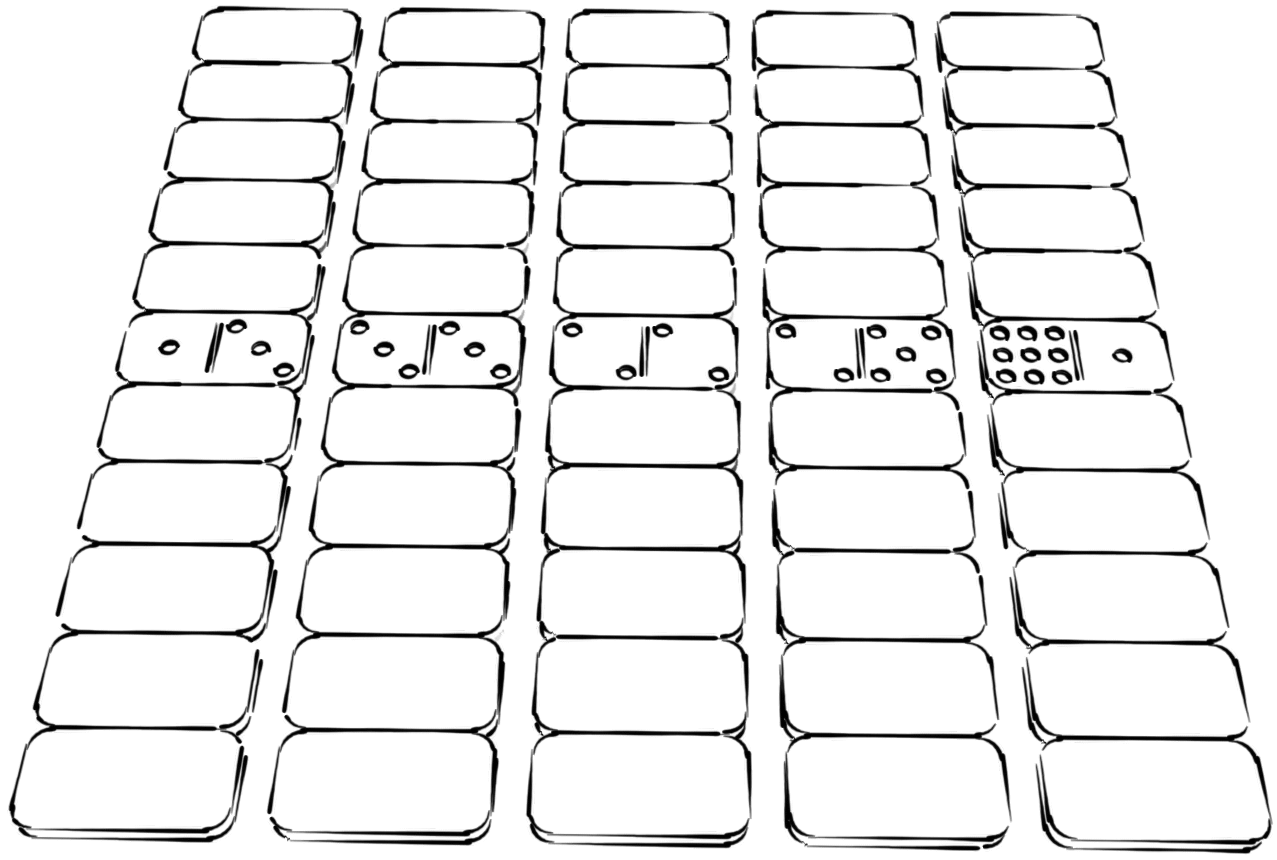
\includegraphics[width = \linewidth]{graphics/dominoes-setup.png}
\caption{Example setup for 2 players. 5 columns of 11 tiles.}
\end{figure}
\subsection{Selection Round}
At this point in the setup process, between 55 and 91 dominoes (depending on player count) should be laid out in neat columns on the table within reach of all the players, and no domines should remain.
Before the game can begin in earnest however, a small selection round is played to give players insight into the available dominoes.

Proceeding clockwise around the table, starting with the youngest player, a player may choose to either 
\begin{itemize} 
\item Reveal one piece in any column
\item Claim a column by taking all the pieces (both flipped and unflipped) for themselves.
\end{itemize}
Play starts once all players have each claimed one column.

\subsubsection{Revealing a Domino}
A player may reveal any one domino in any column they wish.
The revealed domino stays revealed after the fact.
The purpose of this is both to see what column may be benefitial to claim, and gain an insight into what columns to prioritise drawing from later on.

\subsubsection{Claiming a Column}
To claim a column, a player simply takes whichever column on the table, picks up the pieces, and stands them on end (or puts them in holders, etc).
The claimed pieces are hidden from the other players until voluntarily revealed through \textit{Melding} (see Section~\ref{sec:melding}).